\section{Precise Range \ Azimuth Offsets (PRO / PAO \& GPRO / GPAO )}
\label{sec:pro_pao}

\subsection{Evaluation criteria}
\label{sec:pro_pao_criteria}

The pixel offset products provide measurements of local displacements in the range and azimuth directions between a reference and a secondary \acs{cslc}, forming a \acs{cslc} pair. These offsets can be estimated using either phase or amplitude information.

Phase information enables the retrieval of both slant range and azimuth offsets in regions where two distinct looks of the same scene are available. For Sentinel-1 data, this is only feasible within the limited areas of burst overlap, due to the specific geometry of the TOPSAR acquisition mode. Nevertheless, the phase modulation inherent to TOPSAR improves measurement sensitivity, provided that interferometric phase continuity is maintained across adjacent bursts. The residual phase, after conventional processing, can also be exploited to identify motion components in the azimuth direction, offering valuable insight into dynamic surface processes such as glacier flow or landslides. When applicable, phase-based techniques are preferred due to their superior accuracy, which is a consequence of the high sensitivity of the interferometric phase to small displacements.

In cases where phase information is unavailable, decorrelated, or when the displacement to be measured is particularly large (such that phase measurements may underestimate its magnitude due to phase wrapping), amplitude-based methods are employed. These rely on normalized cross-correlation between image patches to estimate local shifts in both range and azimuth directions. Although typically less precise, amplitude-based methods offer broader applicability over heterogeneous surfaces and in low-coherence areas.

The accuracy of the \acs{pro} / \acs{pao} products is critically influenced by the chosen estimation technique, the sensor characteristics, and the properties of the observed scene. For the purpose of this analysis, we assume that ionospheric effects—particularly dispersive phase distortions and group delay—have been properly compensated, either through external ionospheric correction data or via differential techniques that inherently mitigate such disturbances. Indeed, if not correctly addressed, these effects can be erroneously interpreted as surface displacements.

Under this assumption, the remaining sources of error primarily arise from thermal noise, spatial decorrelation, terrain-induced geometric distortions, and limitations of the processing algorithms. These factors affect the precision and reliability of the derived displacement measurements and must be considered in the quality assessment.

To evaluate the achievable accuracy of the \acs{pro} / \acs{pao} products, we analyze the two proposed approaches to estimate range and azimuth shifts (phase-and amplitude-based). In the following, we provide a theoretical examination of the expected quality associated with each method, focusing on their sensitivity and applicability.

\subsection{Theoretical models}
\label{sec:pro_pao_models}

Two methods are proposed for the estimation of pixel offsets in SAR data: phase-based and amplitude-based techniques. Each method is grounded in a distinct theoretical model and is characterized by specific assumptions, performance expectations, and error sources.

\paragraph{Phase-based estimation}

Phase-based methods rely on the coherent phase difference between two complex, co-registered \acs{sar} images (\acs{cslc}). In regions with sufficient coherence $\gamma$, the interferometric phase $\phi$ can be used to retrieve fine displacement information in the range direction, and—under certain constraints—also in the azimuth direction.

For simplicity, we consider two co-registered \acs{sar} images (\acs{cslc}): a reference image $R$ and a slave image $S$. The displacement in the slant range direction, $dr$, corresponding to an area of \(X \times Y\) pixels centered at radar coordinates \((\mathrm{rg}, \mathrm{az})\), can be computed by converting the unwrapped interferometric phase $\phi$ using:

\begin{equation}
dr = \frac{\lambda}{4\pi} \phi
\label{eq:dr_to_phi}
\end{equation}

where $\lambda$ is the radar wavelength, and $\phi$ is the multilooked (i.e., spatially averaged) version of the interferometric phase over the selected window. This formulation assumes that the phase is unambiguous (i.e., properly unwrapped), that atmospheric and ionospheric contributions have been either corrected or strongly mitigated, and, when possible, that the interferogram has been corrected for azimuth displacements.

Evaluating the accuracy of the estimated slant range displacement thus corresponds to assessing the accuracy of the unwrapped interferometric phase. Ignoring unwrapping errors—which, when present, can significantly degrade measurement quality (see Section~\ref{sec:pro_pao_criticalities})—the theoretical accuracy is bounded by the Cramér–Rao lower bound for phase estimation. The standard deviation of the averaged interferometric phase is given by:

\begin{equation}
\sigma_{\phi} = \frac{1}{\sqrt{N}} \cdot \frac{\sqrt{1 - |\gamma|^2}}{|\gamma|}
\label{eq:sigma_phi}
\end{equation}

where $|\gamma|$ is the coherence computed in the \(X \times Y\) window and $N$ is the number of pixels within this window (i.e. $N=X Y$.

The corresponding standard deviation of the estimated slant range displacement is then:

\begin{equation}
\sigma_{dr} = \frac{\lambda}{4\pi} \cdot \frac{1}{\sqrt{N}} \cdot \frac{\sqrt{1 - |\gamma|^2}}{|\gamma|}
\label{eq:sigma_dr}
\end{equation}

This expression highlights that the accuracy of phase-based offset estimation improves with higher coherence and larger averaging windows.

The phase-based technique we propose for estimating the shift in the azimuth direction was originally developed to improve the co-registration of a slave image with respect to its master \cite{Scheiber2000, Prats2012}. It has been extensively demonstrated that this approach enables the reliable detection of subtle motion in the azimuth direction.

To apply this technique, two-look imaging over the same area is required—that is, two nearly simultaneous acquisitions of the same scene with sufficient Doppler centroid separation. The greater the Doppler separation, the higher the sensitivity to azimuthal motion. This condition is particularly well satisfied in Sentinel-1 TOPS mode, where azimuth beam steering introduces significant squint angle diversity within the overlap regions of consecutive bursts. As a result, in the case of Sentinel-1 TOPS mode data, this method provides enhanced sensitivity to azimuthal motion compared to conventional split-beam interferometry, typically applied to Stripmap or ScanSAR acquisitions. A limitation of this approach when applied to Sentinel-1 TOPS mode, however, is that it can only be used in burst overlap regions, which do not cover the entire scene. 

As in the previously discussed case of slant range motion estimation via phase, we now consider two co-registered \acs{sar} images (\acs{cslc}): a reference image $R$ and a slave image $S$. We focus on those regions of the scene where we have two looks with sufficient Doppler separation—namely, the overlap areas between consecutive bursts in Sentinel-1 TOPS acquisitions. For each tile within these regions, consisting of \(X \times Y\) pixels and centered at radar coordinates \((\mathrm{rg}, \mathrm{az})\), we compute the average of the phase difference $\psi$ derived from the two available interferograms as:

\begin{equation}
\psi = \arg\left\{R_{A} \cdot S_{A}^{*} \cdot R_{B} \cdot S_{B}^{*}\right\}
\label{eq:psi}
\end{equation}

Here, $A$ and $B$ identify the two observations with sufficient Doppler separation (in the Sentinel-1 case, these correspond to two consecutive bursts within the same sub-swath). From the phase difference $\psi$, the azimuth displacement $da$ (in meters) can be computed using the relation (\cite{Scheiber1999}):

\begin{equation}
da = \frac{v_{g}}{2\pi \Delta f_{d}} \psi
\label{eq:da_from_psi}
\end{equation}

where $v_{g}$ is the satellite velocity and $\Delta f_{d}$ is the Doppler centroid separation between the two looks. Since $da$ is linearly proportional to the phase difference $\psi$, evaluating the accuracy of the azimuth displacement estimate corresponds to assessing the precision of this phase measurement. Applying the Cramér–Rao lower bound for phase estimation, the standard deviation of the azimuth displacement can be expressed as:

\begin{equation}
\sigma_{da} = \frac{v_{g}}{2\pi \Delta f_{d}} \cdot \frac{1}{\sqrt{N}} \cdot \frac{\sqrt{1 - |\gamma|^2}}{|\gamma|}
\label{eq:sigma_da}
\end{equation}

where $N = X \times Y$ is the number of independent samples used in the averaging, and $|\gamma|$ is the coherence within the tile. 

The following figures graphically illustrate how the accuracy in estimating displacement in both the slant-range and azimuth directions—using the previously described phase-based method—depends on the coherence value ($\gamma$) and the number of pixels N used in the averaging process. Specifically, the first pair of images shows the slant-range accuracy achievable with this method.

In Figure~\ref{fig:rg_accuracy_phase}, the accuracy for displacement estimation in the slant-range direction is presented. The left plot shows the expected accuracy when using \acs{s1} data, while the right plot shows the corresponding accuracy using \acs{rosel} data.

In each plot, the colored curves represent different values of N (i.e., the number of pixels used in the average). It is clearly visible that, for fixed values of N and $\gamma$, the expected accuracy with \acs{s1} is significantly better. This is due to the fact that \acs{s1} operates at a wavelength that is four times shorter than \acs{rosel}'s, resulting in a higher sensitivity to displacement in the slant-range direction.

\begin{figure}[ht!]
\centering
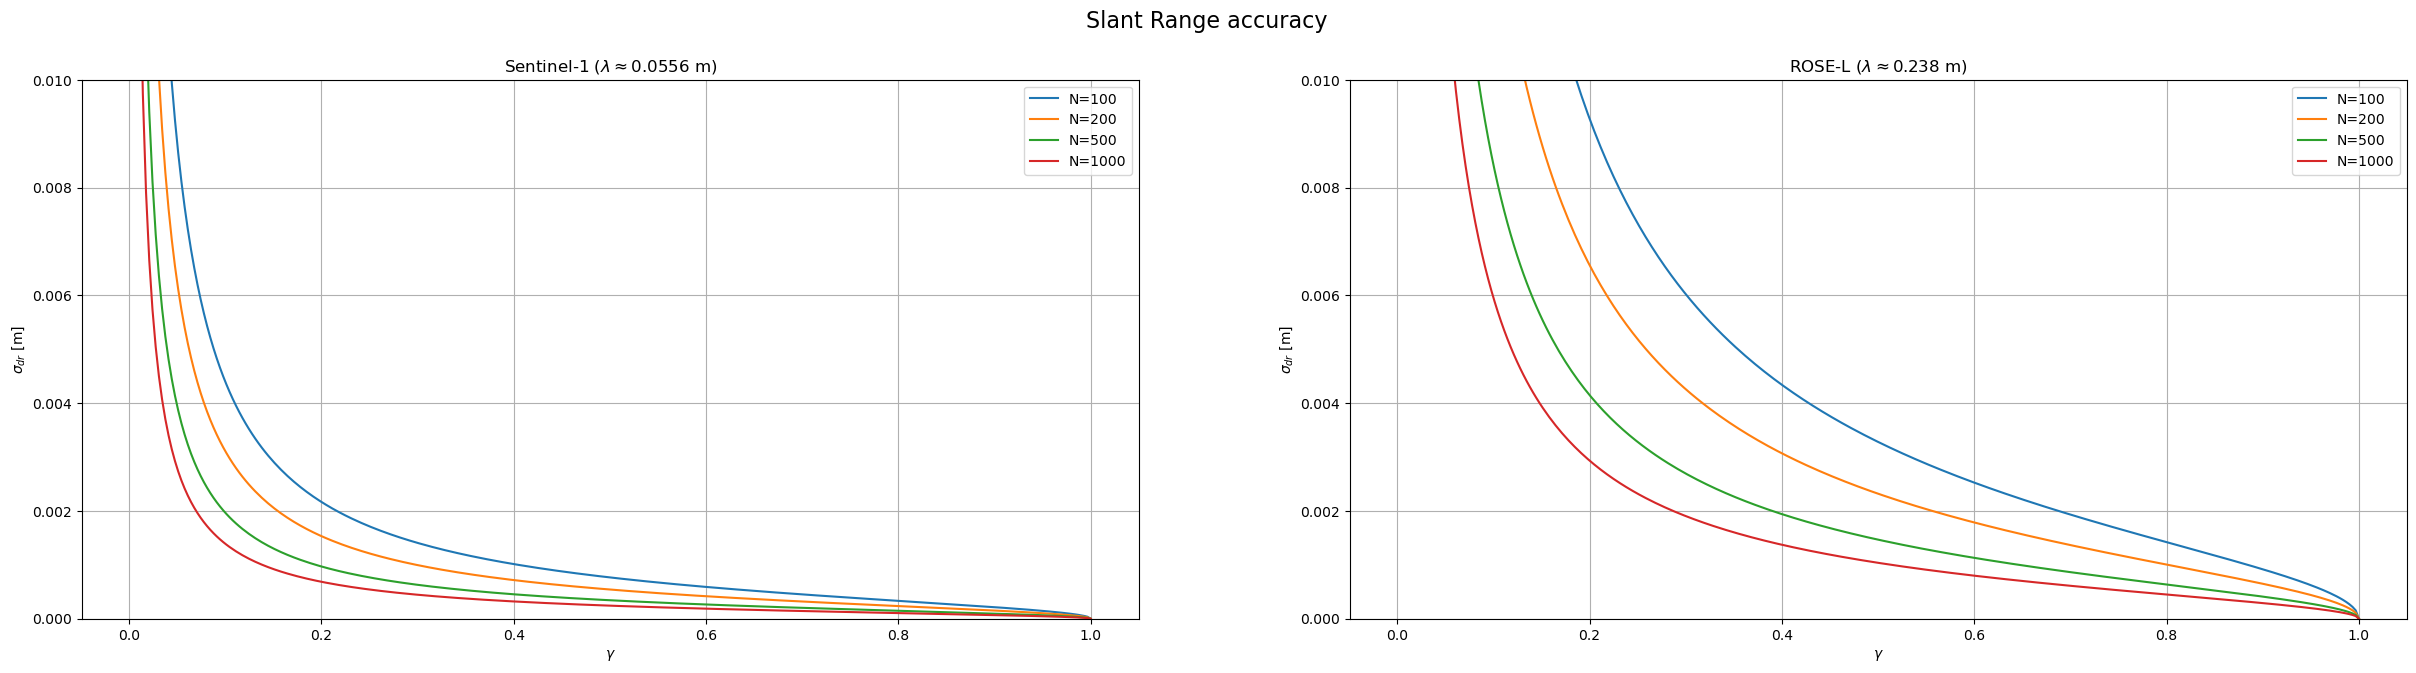
\includegraphics[width=0.9\textwidth]{Figures/pro_pau/rg_accuracy_ph_method.png}
\caption{Slant-range displacement accuracy as a function of coherence ($\gamma$) and the number of pixels N used for averaging, obtained using the phase-based method. The left plot shows results for Sentinel-1, while the right plot shows those for \acs{rosel}. Each colored curve corresponds to a different value of N. Due to its shorter wavelength, Sentinel-1 provides higher sensitivity to displacement, resulting in better accuracy for the same $\gamma$ and N values.}
\label{fig:rg_accuracy_phase}
\end{figure}

Figure~\ref{fig:az_accuracy_phase} illustrates the achievable accuracies in the azimuth direction using the phase-based estimation method, applied to \acs{s1} data (left panel) and \acs{rosel} data (right panel). The curves are plotted as a function of coherence \(|\gamma|\), with different colors corresponding to different values of \(N\), i.e., the number of pixels used in the averaging window. Due to the significantly larger Doppler centroid separation in the burst overlap regions of \acs{s1} acquisitions, the resulting sensitivity to azimuthal motion is notably higher than expected for \acs{rosel}. Consequently, for the same values of \(N\) and coherence, the \acs{s1} case yields substantially better accuracy in azimuth displacement estimation.

\begin{figure}[ht!]
\centering
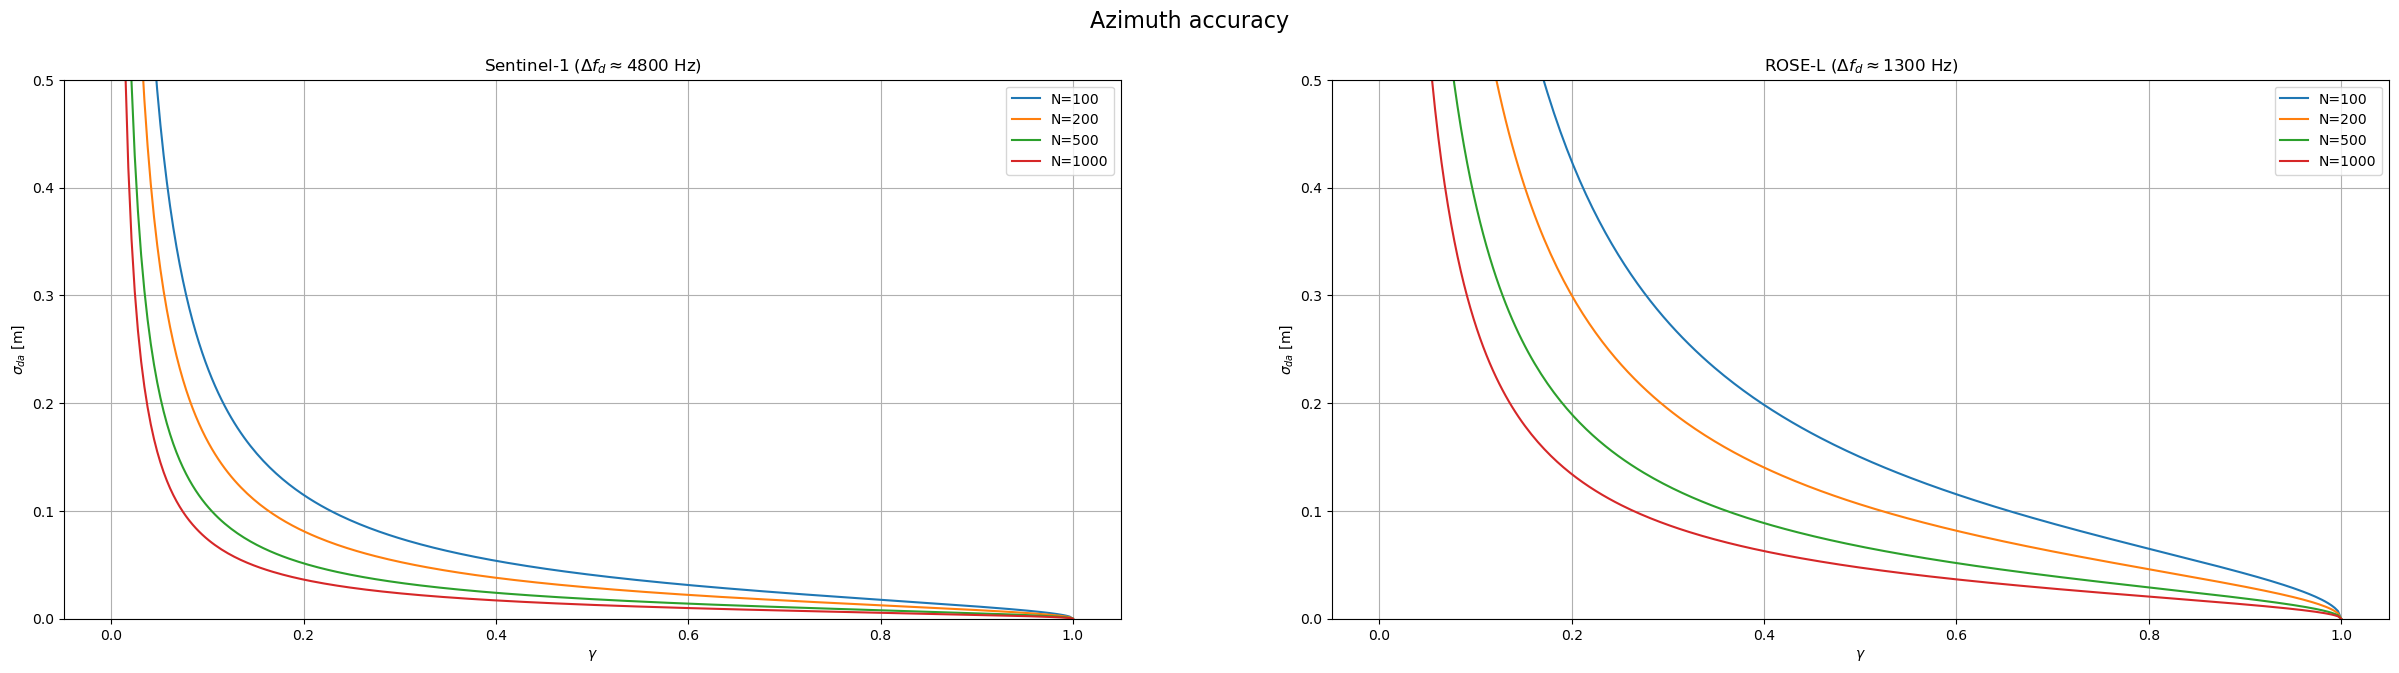
\includegraphics[width=0.9\textwidth]{Figures/pro_pau/az_accuracy_ph_method.png}
\caption{Estimated azimuth displacement accuracy as a function of coherence for different values of \(N\) (number of pixels used in phase averaging), using the phase-based method. Results are shown for \acs{s1} data (left) and \acs{rosel} data (right). The improved Doppler centroid separation in \acs{s1} burst overlaps leads to significantly higher sensitivity to azimuthal motion compared to \acs{rosel}, resulting in lower displacement uncertainty for the same averaging window size and coherence.}
\label{fig:az_accuracy_phase}
\end{figure}

In the following Figure~\ref{fig:example_azimuth_shift_phase} we present some experimental results obtained using \acs{s1} data. As the standard \acs{s1} \acs{slc} products typically provide only a few tens of pixels of overlap between consecutive bursts, and since the phase-based azimuth offset estimation method is only applicable within these overlap regions, we used a custom reprocessed dataset over Greenland. This dataset was specifically modified to increase the overlap between bursts to more than three hundred pixels.

Starting from \acs{cslc} products, we generated an interferogram without applying any Enhanced Spectral Diversity (\acs{esd}) procedure. The phase component corresponding to the displacement in the azimuth direction (as defined by Equation~\ref{eq:psi}) was estimated within the burst overlap regions. Figure~\ref{fig:example_azimuth_shift_phase} shows the interferogram, obtained by mosaicking three consecutive bursts and applying a multilooking factor of 12 (slant range) by 4 (azimuth), along with the phase signal which, when unwrapped and converted to meters, corresponds directly to the azimuth displacement.

This simple experiment demonstrates the applicability of the proposed phase-based approach, as the phase retrieved in the overlap areas shows a coherent pattern. It is not dominated by noise; rather, it clearly contains measurable signal information. At the same time, the bottom panel of Figure~\ref{fig:example_azimuth_shift_phase} highlights one of the primary challenges associated with this method: the requirement for two observations of the same scene with sufficient Doppler separation.

\begin{figure}[ht!]
\centering
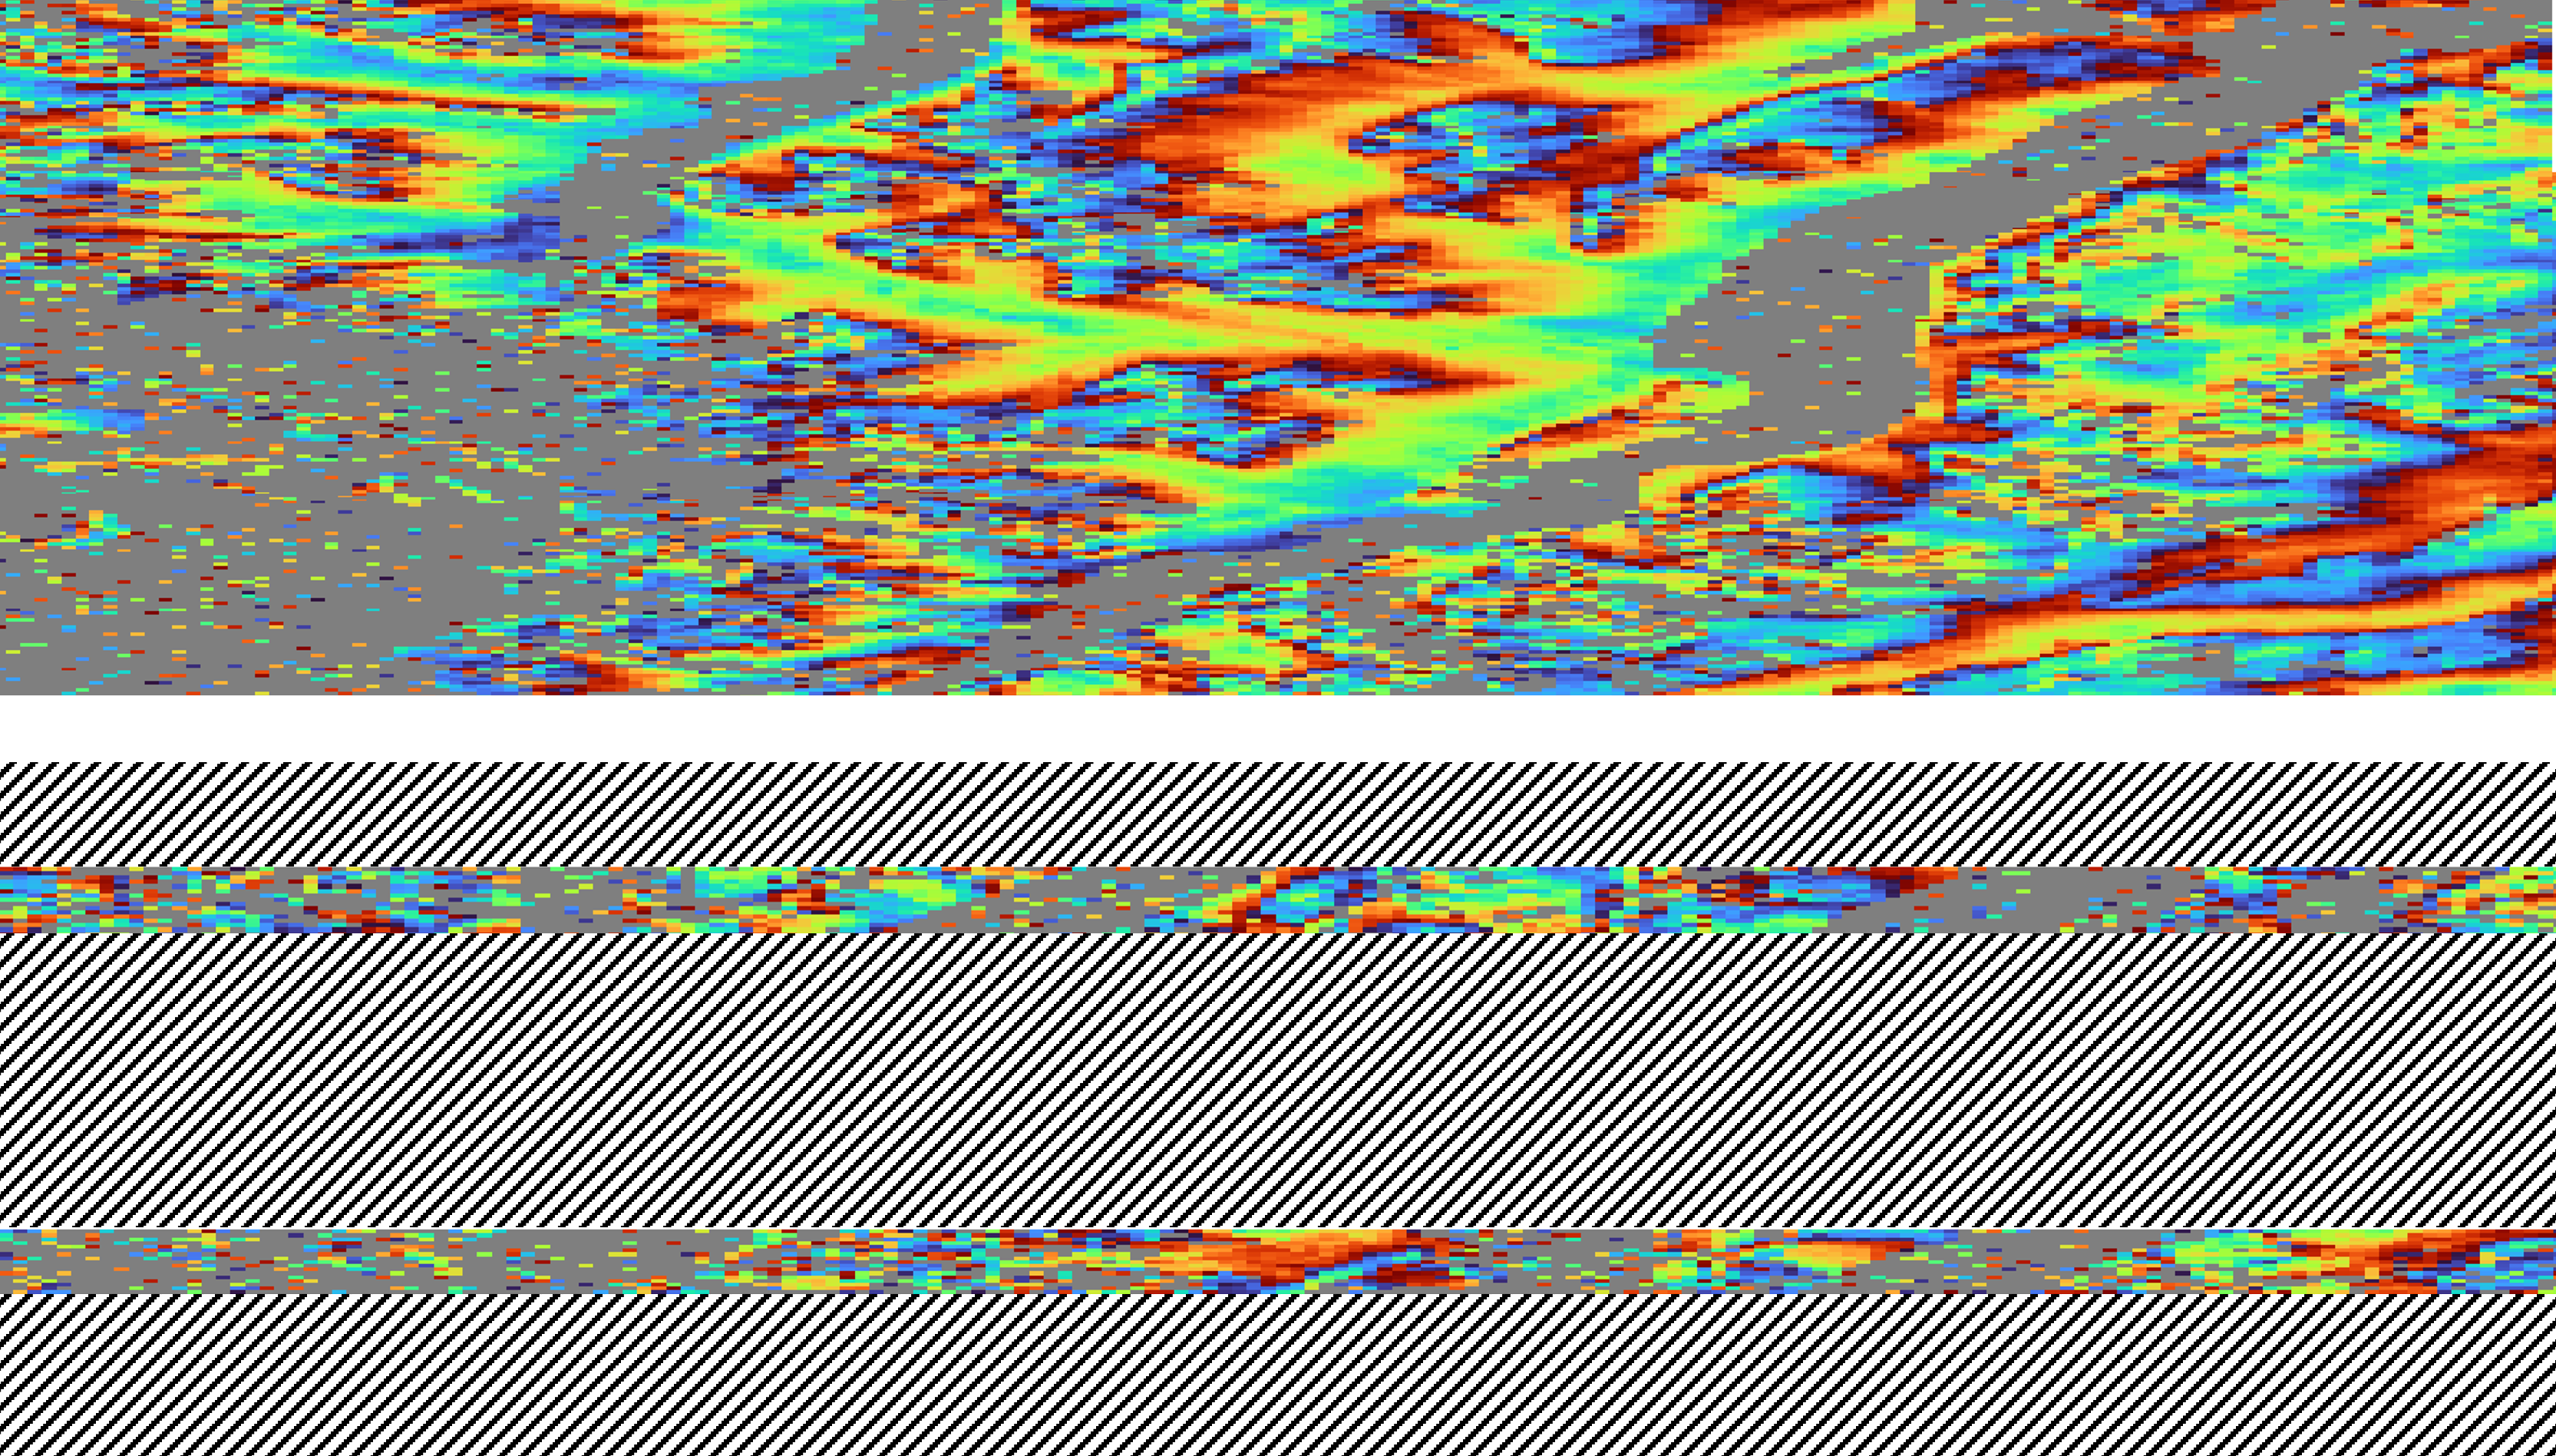
\includegraphics[width=0.9\textwidth]{Figures/pro_pau/example_azimuth_shift_phase.png}
\caption{Top: interferogram obtained by mosaicking three consecutive bursts and applying a multilooking factor of 12 in slant range and 4 in azimuth. The displayed phase component corresponds to the azimuth displacement, which can be unwrapped and converted to meters using Equation~\ref{eq:da_from_psi}. Bottom: estimated azimuth displacement shown only within the burst overlap regions, where phase-based estimation is feasible due to sufficient Doppler separation. Oblique blank areas indicate regions with no burst overlap, where azimuthal shifts cannot be retrieved using this method.}
\label{fig:example_azimuth_shift_phase}
\end{figure}


\paragraph{Amplitude-based estimation using Incoherent Cross-Correlation (ICC)}

In cases where interferometric phase information is unavailable or unreliable—due to temporal decorrelation, low signal-to-noise ratio, or large displacements exceeding the ambiguity limit—displacement estimation can be performed using intensity-only methods. One widely used approach is the Incoherent Cross-Correlation (ICC) method, which relies on measuring the local similarity between image intensities using the Pearson correlation coefficient.

This method estimates the local shift between two co-registered SAR images (\acs{cslc}) by identifying the displacement that maximizes the normalized cross-correlation between small image patches. Let $I_R$ and $I_S$ represent the amplitude images derived from the reference and slave SAR acquisitions, respectively. For each analysis window centered at a pixel with radar coordinates \((\mathrm{rg}, \mathrm{az})\), the normalized cross-correlation surface $C(\Delta r, \Delta a)$ is computed as:

\begin{equation}
C(\Delta r, \Delta a) = \frac{\sum_{x,y} \left(I_R(x, y) - \bar{I}_R\right)\left(I_S(x + \Delta r, y + \Delta a) - \bar{I}_S\right)}{\sqrt{\sum_{x,y} \left(I_R(x, y) - \bar{I}_R\right)^2} \cdot \sqrt{\sum_{x,y} \left(I_S(x + \Delta r, y + \Delta a) - \bar{I}_S\right)^2}}
\label{eq:icc_corr}
\end{equation}

Here, $(x, y)$ are pixel indices within the window of size \(N \times M\), and $\bar{I}_R$, $\bar{I}_S$ are the local mean intensities in the reference and shifted slave patches, respectively. The displacement $(\Delta r, \Delta a)$ that maximizes $C$ corresponds to the estimated local offset in slant range and azimuth directions.

The peak of the cross-correlation surface is typically interpolated with a 2D quadratic or sinc function to obtain sub-pixel accuracy. This method is robust in decorrelated areas or where the phase signal is unreliable, such as vegetated or snow-covered terrain.

De Zan derives the theoretical performance of the ICC estimators under Gaussian-speckle assumptions and constant coherence \cite{DeZan2014}. The variance of the estimated displacement (normalized to the resolution cell) has been shown to depend on the size of the window \(N\) (number of looks) and the coherence \(|\gamma|\). Specifically, for ICC:

\[
\sigma_{\text{ICC}} = \sqrt{\frac{3}{10N}}\frac{\sqrt{2+5\gamma^2-7\gamma^4}}{\pi\gamma^2}
\label{eq:icc_crb}
\]

where:
\begin{itemize}
  \item \(N = N_{\text{looks}} = N_x \times N_y\) is the total number of looks (i.e. total number of pixels in an \(N_x \times N_y\) window).
  \item \(|\gamma|\) is the coherence corresponding to the considered window.
  \item The term is normalized to the resolution cell size (i.e., it yields the standard deviation in pixels).
\end{itemize}

In this expression, \(N\) denotes the number of independent samples (i.e., the number of pixels in the correlation window), and \(|\gamma|\) is the local coherence estimated within the same window. The formula shows that the displacement estimation error increases approximately linearly for relatively high coherence values, while for lower coherence—particularly when \(|\gamma| < 0.6\)—the error rises rapidly. As expected, the error decreases with increasing window size due to averaging effects, but it remains fundamentally limited by the weak signal contrast in low-coherence areas.

In summary, the ICC method offers a flexible and robust approach for estimating displacements in both slant range and azimuth directions when phase-based techniques are not applicable. However, it trades precision for general applicability and should be carefully assessed in terms of its local estimation uncertainty, particularly in low-contrast or spatially homogeneous regions.

Figures~\ref{fig:icc_accuracy_slant} and~\ref{fig:icc_accuracy_azimuth} present the estimated accuracies achievable in slant range and azimuth directions, respectively, using the incoherent cross-correlation (ICC) method. As in the previous figures, the accuracy is shown as a function of coherence \(|\gamma|\), with different curves corresponding to varying values of \(N\), the number of pixels used in the averaging window. The left panels correspond to \acs{s1} system parameters, while the right panels refer to \acs{rosel}.

Unlike the phase-based approach, the theoretical accuracy of ICC is derived in units of pixels. Therefore, to express the results in meters, the slant-range and azimuth pixel spacings specific to \acs{s1} and \acs{rosel} have been applied. The conversion accounts for each sensor's resolution characteristics, ensuring a direct comparison of displacement estimation performance across \acs{sar} systems and methods.

\begin{figure}[ht!]
\centering
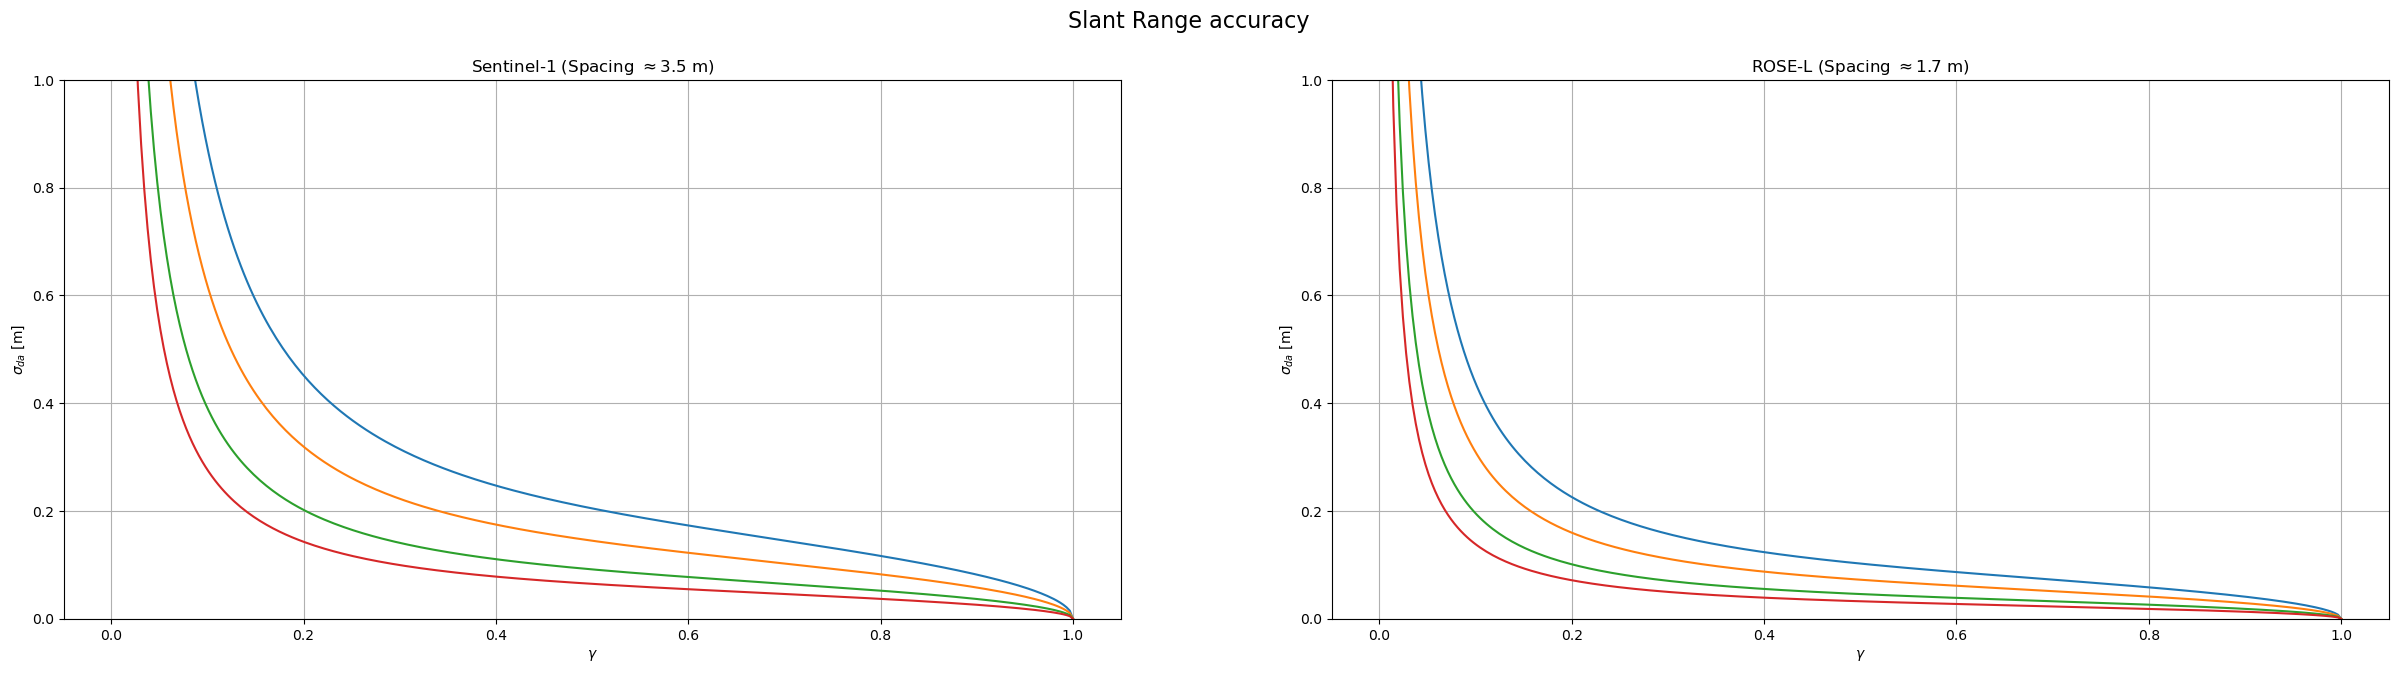
\includegraphics[width=0.9\textwidth]{Figures/pro_pau/rg_accuracy_icc_method.png}
\caption{Estimated slant range displacement accuracy using the incoherent cross-correlation (ICC) method, shown as a function of coherence \(|\gamma|\) for different averaging window sizes \(N\) (represented by color). Left: \acs{s1} configuration. Right: \acs{rosel} configuration. Accuracy is converted from pixels to meters using the corresponding slant-range pixel spacing of each sensor.}
\label{fig:icc_accuracy_slant}
\end{figure}

\begin{figure}[ht!]
\centering
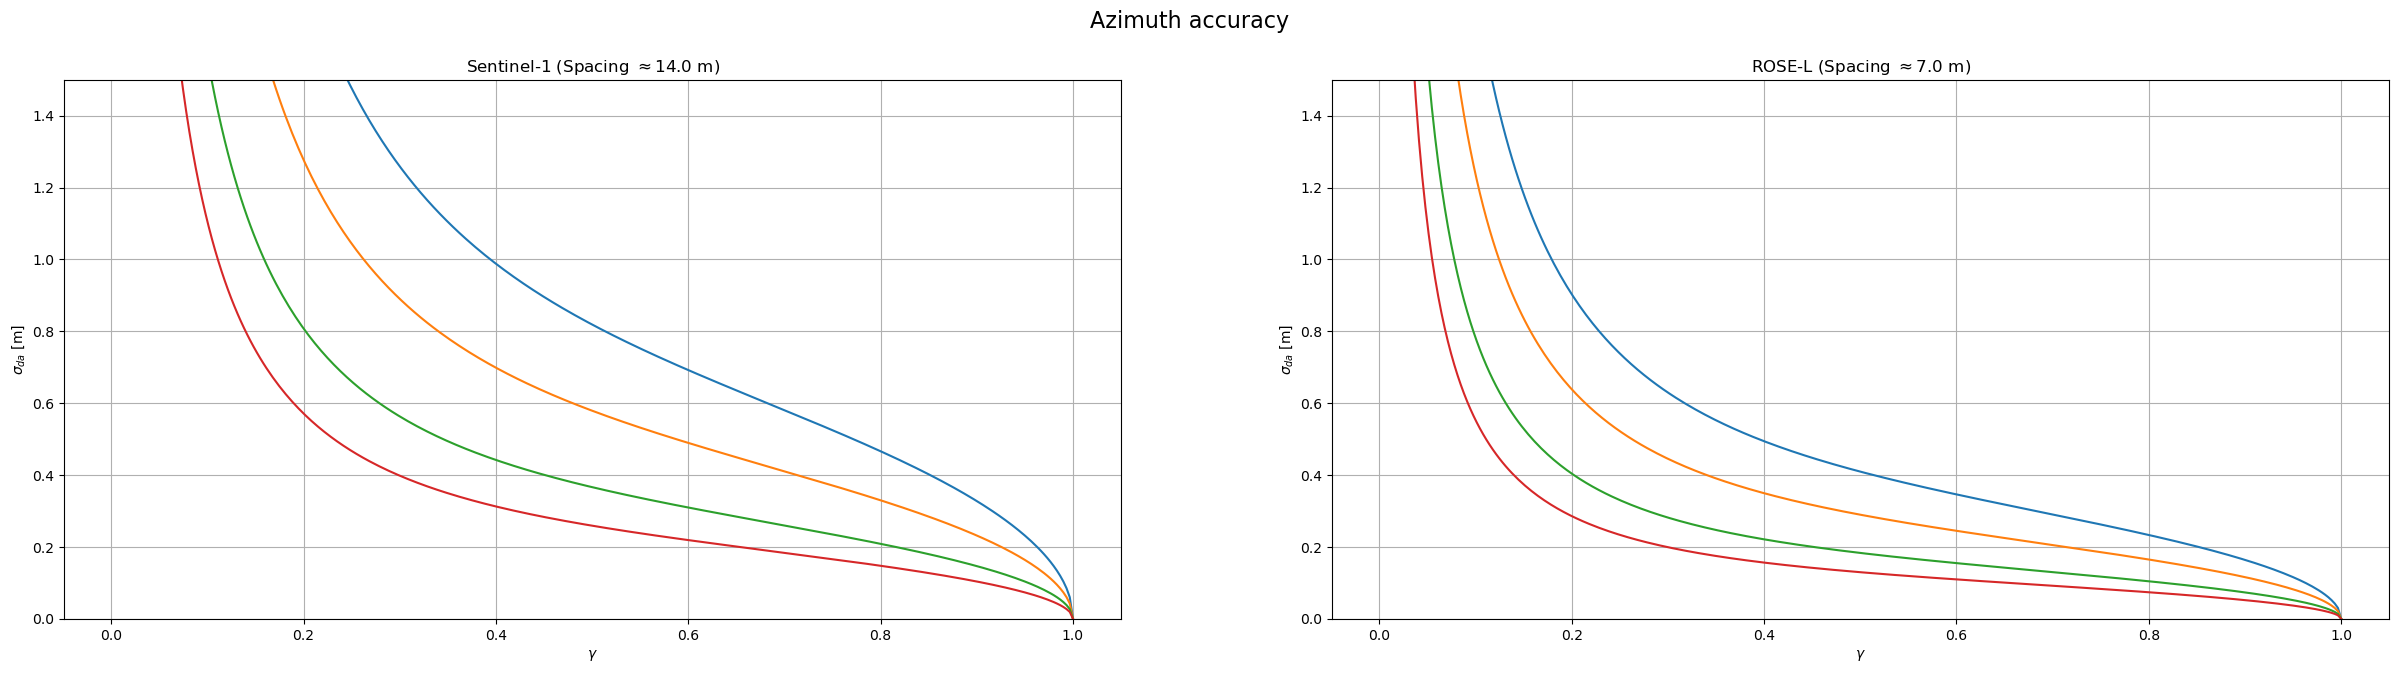
\includegraphics[width=0.9\textwidth]{Figures/pro_pau/az_accuracy_icc_method.png}
\caption{Estimated azimuth displacement accuracy using the incoherent cross-correlation (ICC) method, shown as a function of coherence \(|\gamma|\) for different averaging window sizes \(N\) (represented by color). Left: \acs{s1} configuration. Right: \acs{rosel} configuration. Accuracy is converted from pixels to meters using the respective azimuth pixel spacing of each sensor.}
\label{fig:icc_accuracy_azimuth}
\end{figure}

To illustrate the practical application of the ICC-based method, Figure~\ref{fig:icc_example} shows the estimated displacement field obtained from two \acs{s1} acquisitions over Greenland, separated by 6 days (three consecutive bursts have been used). The displacement vectors were computed using incoherent cross-correlation over a sliding window of 8 pixels in azimuth and 32 pixels in slant range.

Only vectors corresponding to a cross-correlation coefficient greater than 0.4 are shown. Each arrow indicates the direction of the estimated shift, while the color encodes the magnitude of the bidimensional displacement. Despite a notable presence of spurious vectors due to cross-correlation noise—especially in low-texture areas—the majority of the reliable vectors have low magnitude, supporting the assumption of negligible surface motion in this region during the observation period.

\begin{figure}[ht!]
\centering
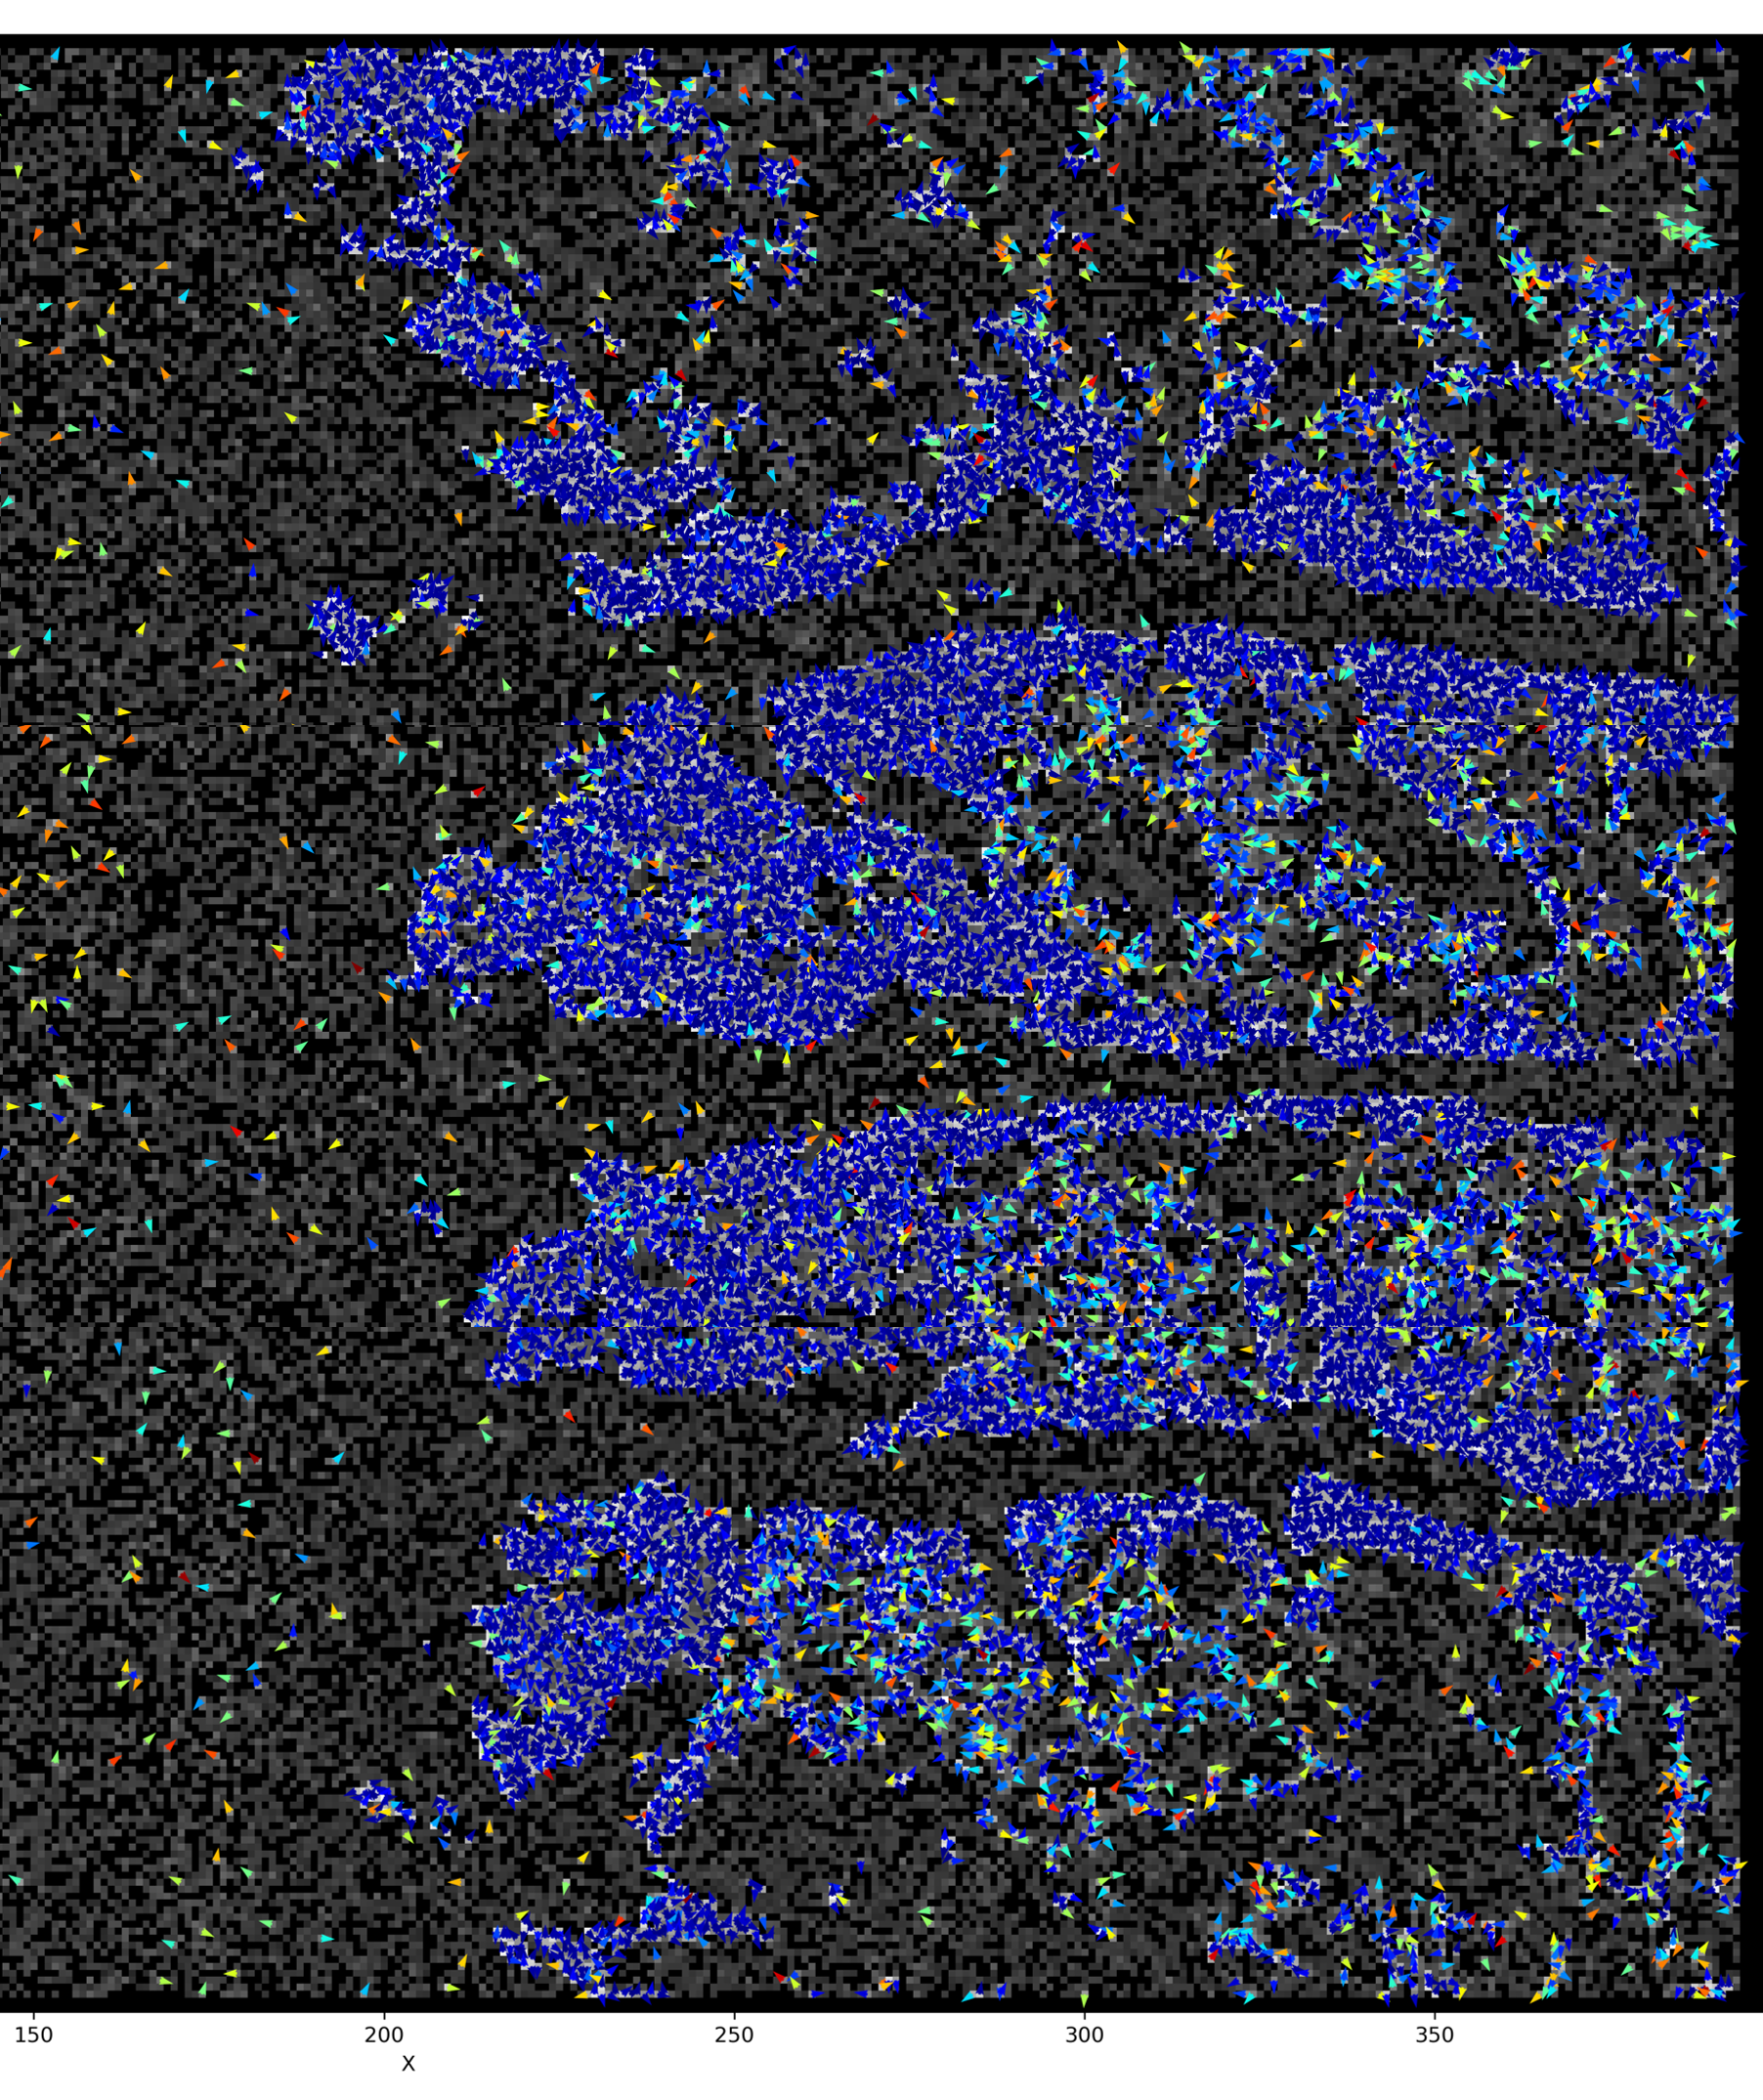
\includegraphics[width=0.8\textwidth]{Figures/pro_pau/icc_example.png}
\caption{Displacement field estimated using the ICC-based method from two Sentinel-1 acquisitions over Greenland, 6 days apart. The image combines three consecutive bursts. Vectors were computed using a cross-correlation window of 8 pixels (azimuth) by 32 pixels (slant range), and only those with a correlation coefficient greater than 0.4 are displayed. Arrow direction indicates the direction of motion, while arrow color represents the magnitude of the estimated bidimensional displacement.}
\label{fig:icc_example}
\end{figure}

\subsection{Computational performance}
\label{sec:pro_pao_computation}

The computational performance of the pixel offset estimation workflow depends significantly on the selected method—phase-based or amplitude-based (ICC)—and on system-specific parameters such as data resolution, overlap area, and window size.

\paragraph{Phase-based estimation}

The phase-based method, which relies on the coherent combination of complex SAR images, is computationally efficient in terms of per-pixel cost but limited in spatial applicability due to the requirement for burst overlap with sufficient Doppler separation. Key steps such as interferogram formation and multilooking are highly optimized and can be parallelized across image tiles. The most computationally intensive component is typically the phase unwrapping stage, particularly in low-coherence regions. However, this cost is mitigated by the fact that significant multilooking is typically applied, which reduces the number of resolution cells to unwrap. As a result, the unwrapping step remains tractable, and the overall processing can be completed in reasonable time. On standard multi-core CPU systems, processing times range from a few seconds to tens of minutes per scene.

\paragraph{ICC-based estimation}

The incoherent cross-correlation (ICC) method can be computationally demanding, especially when applied to large swaths of data. The core of the algorithm involves computing normalized cross-correlation over a sliding window for each valid pixel, followed by sub-pixel peak interpolation. This procedure is repeated independently for each direction (range and azimuth) and can be parallelized both spatially and across bursts. However, memory and I/O demands are non-negligible, particularly when using large windows or high-resolution data such as from \acs{rosel}. The ICC approach scales with the number of search positions and with the window size, making optimization strategies—such as coarse-to-fine search, fast correlation via FFT, and GPU acceleration—highly beneficial. 

\subsection{Criticalities and weakness}
\label{sec:pro_pao_criticalities}

Both phase-based and amplitude-based (ICC) displacement estimation methods are subject to several potential sources of error that must be carefully addressed to ensure reliable measurements. One of the most critical factors affecting the accuracy of displacement estimates—particularly in the slant range direction, but also to a lesser extent in the azimuth direction—is the presence of atmospheric propagation delays.

Tropospheric and ionospheric delays can introduce systematic biases in the measured phase, potentially leading to erroneous displacement estimates. This is especially critical for L-band SAR systems (e.g., \acs{rosel}), where ionospheric effects are more pronounced. Therefore, a fundamental prerequisite for producing reliable \acs{pro} and \acs{pao} products is mitigation of these atmospheric disturbances. Correction strategies include the use of external data—such as ECMWF-based tropospheric delay models or ionospheric delay maps derived from GNSS—or data-driven approaches like the split-spectrum technique, which is particularly effective for isolating ionospheric effects. Regardless of the method used, it is essential to ensure that atmospheric contributions are minimized prior to performing the displacement estimation steps.

In the case of phase-based displacement estimation, an additional critical step is phase unwrapping. This process, which reconstructs the absolute phase from its modulo-\(2\pi\) observations, is inherently complex and highly sensitive to coherence. In areas of low coherence, unwrapping algorithms are prone to errors that can cause entire phase jumps to be missed. Such errors are not local: they can propagate spatially, affecting large areas and introducing displacement artifacts that significantly exceed the noise levels or residual atmospheric effects.

This makes phase unwrapping one of the most failure-prone components in the processing chain when applying the phase-based method. In practice, unwrapping errors can produce large-scale misestimation of displacements, undermining the scientific validity of the results. For this reason, special attention must be paid to both the quality of the coherence map and the robustness of the unwrapping algorithm before accepting phase-derived displacement results as reliable.